
\documentclass[11pt,letterpaper]{article}
\usepackage[margin=0.76in,top=0.72in,bottom=0.78in]{geometry}
\usepackage[T1]{fontenc}
\usepackage[utf8]{inputenc}
\usepackage{lmodern}
\usepackage{microtype}
\usepackage{amsmath,amssymb,mathtools}
\usepackage{booktabs,tabularx,longtable,array,multirow}
\usepackage{enumitem}
\usepackage{xcolor}
\usepackage{graphicx}
\usepackage{tikz}
\usetikzlibrary{arrows.meta,positioning,calc,shapes.geometric,fit,backgrounds,decorations.pathmorphing}
\usepackage[skins,breakable]{tcolorbox}
\usepackage{listings}
\usepackage{fancyhdr}
\usepackage{titlesec}
\usepackage{tocloft}
\usepackage{hyperref}
\usepackage{caption}
\usepackage{float}
\usepackage{needspace}

\definecolor{Ivory}{HTML}{FBF7EC}
\definecolor{Navy}{HTML}{0D1B2E}
\definecolor{Navy2}{HTML}{10233D}
\definecolor{Gold}{HTML}{B58A22}
\definecolor{SoftGold}{HTML}{EBD9A8}
\definecolor{MutedBlue}{HTML}{5B6B86}
\definecolor{PaleBlue}{HTML}{EAF2F8}
\definecolor{PaleGreen}{HTML}{E6F5ED}
\definecolor{PaleViolet}{HTML}{EEEAF9}
\definecolor{PaleRose}{HTML}{FAEAEA}
\definecolor{Ink}{HTML}{172033}
\definecolor{CodeBg}{HTML}{F8F4E8}
\pagecolor{Ivory}
\color{Ink}
\hypersetup{colorlinks=true,linkcolor=Navy,citecolor=Navy,urlcolor=Navy,pdftitle={Merkle Roots for the Validated Skill Graph v114},pdfauthor={Vincent Boucher},pdfsubject={GoalOS, Validated Skill Graph, Merkle roots},pdfkeywords={GoalOS, Merkle roots, Validated Skill Graph, Evidence Docket, Chronicle, AGI Jobs, Ethereum}}
\setlength{\parindent}{0pt}
\setlength{\parskip}{6pt}
\setlength{\headheight}{22pt}
\emergencystretch=3em
\sloppy
\renewcommand{\baselinestretch}{1.04}
\pagestyle{fancy}
\fancyhf{}
\lhead{\footnotesize\scshape GoalOS: Merkle Roots for the Validated Skill Graph}
\rhead{\footnotesize\scshape Montreal.AI Research}
\cfoot{\footnotesize \thepage}
\renewcommand{\headrulewidth}{0.4pt}
\renewcommand{\headrule}{\hbox to\headwidth{\color{SoftGold}\leaders\hrule height \headrulewidth\hfill}}
\titleformat{\section}{\Large\bfseries\scshape\color{Navy}}{\thesection}{0.6em}{}[\vspace{-3pt}{\color{Gold}\titlerule[0.5pt]}]
\titleformat{\subsection}{\large\bfseries\color{Navy}}{\thesubsection}{0.6em}{}
\titleformat{\subsubsection}{\normalsize\bfseries\color{Navy}}{\thesubsubsection}{0.6em}{}
\captionsetup{font=small,labelfont={bf,color=Navy},textfont=it}
\setlist[itemize]{leftmargin=1.4em,itemsep=2pt,topsep=3pt}
\setlist[enumerate]{leftmargin=1.7em,itemsep=2pt,topsep=3pt}
\newcolumntype{Y}{>{\raggedright\arraybackslash}X}
\newcommand{\domain}[1]{\texttt{#1}}
\newcommand{\hash}{\mathsf{H}}
\newcommand{\canon}{\mathsf{canon}}
\newcommand{\Root}{\mathsf{Root}}
\newcommand{\Leaf}{\mathsf{Leaf}}
\newcommand{\VSG}{\mathsf{VSG}}
\newcommand{\Chronicle}{\mathsf{Chronicle}}
\newcommand{\ChroniclePass}{\mathsf{ChroniclePass}}
\newcommand{\Admit}{\mathsf{Admit}}
\newcommand{\Verify}{\mathsf{Verify}}
\newcommand{\GraphRoot}{\mathsf{graphEpochRoot}}
\newcommand{\SkillRoot}{\mathsf{skillNodeRoot}}
\newcommand{\EvidenceRoot}{\mathsf{evidenceDocketRoot}}
\newcommand{\BundleRoot}{\mathsf{proofBundleRoot}}
\newcommand{\PolicyRoot}{\mathsf{policyRoot}}
\newcommand{\AttestationRoot}{\mathsf{attestationRoot}}
\newcommand{\RevocationRoot}{\mathsf{revocationRoot}}
\newcommand{\SupersessionRoot}{\mathsf{supersessionRoot}}
\newcommand{\MetadataRoot}{\mathsf{metadataRoot}}

% Light-only callout boxes: no dark fills; all body text remains dark and printable.
\newtcolorbox{thesisbox}[1][]{enhanced,breakable,colback=white!82!Ivory,colframe=Gold,coltext=Ink,arc=4pt,boxrule=0.65pt,left=10pt,right=10pt,top=10pt,bottom=9pt,title=#1,coltitle=Navy,fonttitle=\bfseries\scshape,attach boxed title to top left={yshift=-2mm,xshift=3mm},boxed title style={colback=SoftGold!92!white,colframe=Gold,arc=2pt}}
\newtcolorbox{lawbox}[1][]{enhanced,breakable,colback=CodeBg,colframe=Gold,coltext=Ink,arc=4pt,boxrule=0.55pt,left=10pt,right=10pt,top=10pt,bottom=9pt,title=#1,coltitle=Navy,fonttitle=\bfseries\scshape,attach boxed title to top left={yshift=-2mm,xshift=3mm},boxed title style={colback=SoftGold!92!white,colframe=Gold,arc=2pt}}
\newtcolorbox{bluebox}[1][]{enhanced,breakable,colback=PaleBlue,colframe=MutedBlue,coltext=Ink,arc=4pt,boxrule=0.5pt,left=9pt,right=9pt,top=8pt,bottom=8pt,title=#1,coltitle=Navy,colbacktitle=PaleBlue,fonttitle=\bfseries\scshape,boxed title style={colback=PaleBlue,colframe=MutedBlue}}
\newtcolorbox{greenbox}[1][]{enhanced,breakable,colback=PaleGreen,colframe=teal!60!black,coltext=Ink,arc=4pt,boxrule=0.5pt,left=9pt,right=9pt,top=8pt,bottom=8pt,title=#1,coltitle=Navy,colbacktitle=PaleGreen,fonttitle=\bfseries\scshape,boxed title style={colback=PaleGreen,colframe=teal!60!black}}
\newtcolorbox{redbox}[1][]{enhanced,breakable,colback=PaleRose,colframe=red!55!black,coltext=Ink,arc=4pt,boxrule=0.5pt,left=9pt,right=9pt,top=8pt,bottom=8pt,title=#1,coltitle=Navy,colbacktitle=PaleRose,fonttitle=\bfseries\scshape,boxed title style={colback=PaleRose,colframe=red!55!black}}
\newtcolorbox{protocolbox}[1][]{enhanced,breakable,colback=white!70!Ivory,colframe=SoftGold,coltext=Ink,arc=4pt,boxrule=0.5pt,left=9pt,right=9pt,top=8pt,bottom=8pt,title=#1,coltitle=Navy,colbacktitle=SoftGold!92!white,fonttitle=\bfseries\scshape,boxed title style={colback=SoftGold!92!white,colframe=Gold}}

\lstdefinelanguage{json}{basicstyle=\scriptsize\ttfamily,showstringspaces=false,breaklines=true,frame=single,rulecolor=\color{SoftGold},backgroundcolor=\color{CodeBg},string=[s]{"}{"},stringstyle=\color{Navy},comment=[l]{//},commentstyle=\color{MutedBlue},morecomment=[s]{/*}{*/},numbers=none}
\lstset{basicstyle=\scriptsize\ttfamily,breaklines=true,columns=fullflexible,keepspaces=true,frame=single,rulecolor=\color{SoftGold},backgroundcolor=\color{CodeBg}}

\begin{document}

\begin{titlepage}
\thispagestyle{empty}
\begin{center}
\vspace*{0.55in}
{\small\scshape\color{Gold} Montreal.AI Research \quad $\diamond$ \quad GoalOS Protocol Note Series}\par
\vspace{0.9in}
{\fontsize{28}{31}\selectfont\bfseries\color{Navy} Merkle Roots for the\par Validated Skill Graph}\par
\vspace{0.22in}
{\large\itshape\color{MutedBlue} Production Merkle Epoch Roots, Chronicle-Gated Memory,\par Selective Disclosure, ENS-Gated Writes, and Root-Verified Capability}\par
\vspace{0.55in}
{\color{Gold}\rule{3.0in}{0.55pt}}\par
\vspace{0.42in}
{\Large\bfseries Vincent Boucher}\par
\vspace{0.07in}
{\large President, QUEBEC.AI \& MONTREAL.AI}\par
\vspace{0.34in}
{\small Research Edition v4.0 / GoalOS V114 \quad | \quad Publication-safe, claim-bounded}\par
\vfill
\begin{thesisbox}[Core Thesis]
Merkle roots are one of the most useful primitives for the Validated Skill Graph because they let GoalOS commit to large, private, evolving sets of skills, evidence, ProofBundles, policies, attestations, encrypted-capsule references, and graph state with a compact, auditable root. A future mission may trust only what is both Chronicle-admitted and root-verifiable.
\end{thesisbox}
\vspace{0.2in}
{\itshape AI creates output. GoalOS creates proof. Merkle roots make proof state compact, inspectable, and difficult to silently rewrite.}\par
\vspace{0.45in}
{\color{SoftGold}\rule{\textwidth}{0.5pt}}\par
\end{center}
\end{titlepage}

\begingroup
\small
\setlength{\cftbeforesecskip}{2pt}
\setlength{\cftbeforesubsecskip}{0pt}
\tableofcontents
\endgroup
\newpage

\begin{abstract}
The Validated Skill Graph is a proof-carrying memory substrate for autonomous AI work: candidate output becomes reusable capability only after Proof Debt is retired, AGI Jobs return evidence, an Evidence Docket aggregates proof, and Chronicle admits a scoped skill. This paper argues that Merkle roots are the natural commitment primitive for that graph. A Merkle-native Validated Skill Graph represents skills, graph edges, Evidence Dockets, ProofBundles, policies, attestations, revocations, supersessions, encrypted capsule references, and metadata as domain-separated leaves. It derives typed subroots and binds them into a single graph epoch root. The root can be committed on-chain while private intelligence remains encrypted, off-chain, or zero-knowledge-proven. The result is a compact, tamper-evident, inclusion-verifiable substrate for reusable capability. We formalize canonicalization, domain separation, root construction, inclusion proofs, root continuity, Chronicle gating, direct-agent authorization, privacy boundaries, zero-knowledge compatibility, threat models, conformance levels, and evaluation tests. The central claim is architectural and falsifiable: durable capability memory should not be a transcript, prompt library, or mutable database; it should be a proof-gated graph whose admitted state is committed by cryptographic roots and whose private contents remain protected.
\end{abstract}

\begin{lawbox}[Executive Compression]
\textbf{Problem.} AI systems produce abundant output, but institutions need evidence-backed memory. \textbf{Solution.} Chronicle admits validated skills; Merkle roots commit the admitted state. \textbf{Principle.} Store roots, proofs, ciphertext commitments, and controlled pointers - not plaintext private intelligence. \textbf{Outcome.} Future missions improve only from skills that are Chronicle-admitted, scope-compatible, and root-verifiable.
\end{lawbox}


\section{One-Page Protocol Standard}
\begin{lawbox}[The Four-Layer Law]
\textbf{State is not authority.} A Merkle root proves that an exact graph state existed. \textbf{Proof is not privacy leakage.} The public layer may store roots, hashes, attestations, and pointers while private intelligence remains encrypted or off-chain. \textbf{Inclusion is not truth.} Chronicle, Evidence Dockets, ProofBundles, validators, proof levels, and rollback conditions decide whether an included object earns reuse authority. \textbf{Memory is not a transcript.} Only proof-admitted capability may influence future missions.
\end{lawbox}

\begin{table}[H]
\small
\centering
\begin{tabularx}{\textwidth}{p{1.35in}Y Y Y}
\toprule
Layer & Object & What it proves & What it does not prove\\
\midrule
Capability & Validated Skill & A scoped method has passed a policy gate for a defined use envelope. & Universal correctness or unrestricted reuse.\\
Evidence & Evidence Docket / ProofBundle & The claim has support, replay material, validator route, and boundary notes. & Legal certification or production authorization.\\
Commitment & Merkle root / graphEpochRoot & The exact canonical graph state and selected leaves are tamper-evidently committed. & Truth, safety, legality, or quality by itself.\\
Authority & Chronicle Gate / policy & The capability may influence future missions under recorded scope. & Immunity from drift, deployment risk, or liability.\\
\bottomrule
\end{tabularx}
\caption{The Merkle root is a commitment layer; Chronicle is the authority layer. Keeping the two separate prevents hash inclusion from becoming accidental institutional trust.}
\end{table}

\begin{figure}[H]
\centering
\resizebox{\textwidth}{!}{\begin{tikzpicture}[font=\scriptsize, >=Latex, node distance=0.62cm]
\tikzset{box/.style={draw=Navy, rounded corners=4pt, align=center, minimum width=1.55in, minimum height=.42in, fill=white}, p/.style={box, fill=PaleBlue}, e/.style={box, fill=PaleGreen}, c/.style={box, fill=SoftGold!55}, a/.style={box, fill=PaleViolet}}
\node[p] (priv) {Private capability\\method, traces, reviewer notes};
\node[e, right=of priv] (evi) {Proof artifacts\\Docket, bundles, attestations};
\node[c, right=of evi] (root) {Commitment state\\typed Merkle forest};
\node[a, right=of root] (auth) {Authority state\\Chronicle decision};
\node[e, right=of auth] (future) {Future mission\\bounded capability prior};
\foreach \x/\y in {priv/evi,evi/root,root/auth,auth/future} \draw[->,thick,Navy] (\x)--(\y);
\draw[->,dashed,thick,Gold!80!black] (root.south) .. controls +(0,-.45) and +(0,-.45) .. node[below]{selective disclosure proofs} (evi.south);
\draw[->,dashed,thick,red!60!black] (auth.north) .. controls +(0,.38) and +(0,.38) .. node[above]{repair / reject / quarantine if gate fails} (evi.north);
\node[fit=(priv)(future), draw=SoftGold, rounded corners=8pt, inner sep=.16in] {};
\end{tikzpicture}}
\caption{State, proof, commitment, and authority are separated. Merkle roots make the graph auditable; Chronicle decides what earns memory.}
\end{figure}

\section{Introduction}
Modern AI systems can generate text, code, plans, traces, claims, and tool actions at extraordinary scale. The bottleneck is no longer generation alone; it is deciding what deserves memory, reuse, settlement, propagation, or future-mission influence. GoalOS addresses that bottleneck with a proof-to-capability loop:
\[
\begin{aligned}
&\text{Objective} \to \text{Proof Mission} \to \text{AGI Jobs} \to \text{Evidence} \to \text{Chronicle}\\
&\to \text{Validated Skill} \to \text{On-chain Graph Root} \to \text{Future Mission Improvement}.
\end{aligned}
\]

The loop treats unsupported claims as Proof Debt; Proof Debt becomes AGI Jobs; AGI Jobs return ProofBundles; ProofBundles update an Evidence Docket; Chronicle decides what may become durable memory; admitted results become Validated Skills; and the Validated Skill Graph provides future missions with scoped reusable capability.

This paper focuses on one primitive inside that architecture: the Merkle root. A Merkle root compresses a set of leaves into a single digest while preserving efficient membership proofs and tamper detection. For a Validated Skill Graph, this primitive is unusually valuable because the graph is large, dynamic, partially private, and audit-sensitive. A reviewer should be able to verify that a skill, evidence item, ProofBundle, validator attestation, policy object, revocation, or supersession was included in a committed graph state without requiring the entire private graph to be exposed.

\begin{thesisbox}[Operating Law]
A skill may influence a future mission only if it is admitted by Chronicle and bound to an auditable graph-root state. A root is not the skill. It is the tamper-evident public commitment to the skill graph state.
\end{thesisbox}

\section{Contributions}
This paper makes twelve contributions.
\begin{enumerate}
\item \textbf{Merkle-native VSG model.} A formal representation of the Validated Skill Graph as a forest of typed Merkle roots.
\item \textbf{Domain-separated leaf hashing.} A deterministic scheme for skill, edge, evidence, ProofBundle, policy, attestation, revocation, supersession, metadata, and graph-root leaves.
\item \textbf{Graph-epoch composition.} A method for binding multiple typed roots into one graph epoch root with chain, registry, agent, epoch, policy, snapshot, and previous-root context.
\item \textbf{Chronicle-root law.} A rule that only Chronicle-admitted skills may be committed as future-mission-influencing capability.
\item \textbf{Selective disclosure and review paths.} Reviewer workflows for verifying that a claim, skill, or evidence item is or is not part of a committed state.
\item \textbf{Privacy-preserving on-chain boundary.} A root-and-proof pattern that supports encrypted capsules and zero-knowledge receipts while avoiding plaintext private intelligence on-chain.
\item \textbf{Direct-agent authorization.} An ENS-style direct \texttt{*.agent.agi.eth} authorization model for graph-root writers.
\item \textbf{Lifecycle semantics.} Root continuity, supersession, revocation, retirement, and stale-root protections.
\item \textbf{Threat and falsification model.} Tests for tampering, equivocation, unauthorized writes, replay, stale roots, memory contamination, and serialization drift.
\item \textbf{Production artifact standard.} JSON schemas, algorithms, acceptance tests, conformance levels, and UI requirements for implementing Merkle roots inside GoalOS.
\item \textbf{V107-compatible registry surface.} Contract-level methods for \texttt{computeLeaf}, \texttt{verifyEpochLeaf}, \texttt{commitGraphEpoch}, expected-root matching, epoch-number enforcement, and previous-root continuity.
\item \textbf{Reviewer-centered verification UX.} A practical review path that shows non-technical operators what a Merkle proof proves, what remains unproven, and when a new proof mission is required.
\end{enumerate}

\section{System Positioning}
The proof-loop doctrine can be summarized as follows: start with the objective, not the agent; keep the workbench empty until Proof Debt exists; generate only custom AGI Jobs; make Evidence Dockets inspectable; use Chronicle as the memory firewall; and store proof roots rather than plaintext private intelligence. This is the operating rule that turns autonomous work into proof and proof into reusable capability.

A Validated Skill is not a note. It is a governed capability object. It has scope, method, evidence, tests, validators, risk boundaries, policy, version, rollback conditions, and utility. A Validated Skill Graph stores those skills and the policy-scoped relationships between them: reuse, compose, teach, package, audit, retire, supersede, and future-prior influence.

The graph has three distinct layers:
\begin{enumerate}
\item \textbf{Private capability layer:} methods, reviewer notes, traces, sensitive data, internal tooling details, and private evidence.
\item \textbf{Proof artifact layer:} ProofBundles, Evidence Docket entries, replay manifests, validator attestations, and Chronicle decisions.
\item \textbf{Commitment layer:} Merkle roots, content hashes, ZK proof hashes, policy hashes, direct-agent identity, and append-only root history.
\end{enumerate}
Merkle roots are the bridge between the proof artifact layer and the commitment layer.

\begin{figure}[H]
\centering
\resizebox{\textwidth}{!}{\begin{tikzpicture}[font=\scriptsize, node distance=0.55cm, >=Latex]
\tikzset{box/.style={draw=Navy, rounded corners=3pt, minimum width=1.03in, minimum height=0.38in, align=center, fill=white}, goldbox/.style={box, fill=SoftGold!55}, bluebox/.style={box, fill=PaleBlue}, greenbox/.style={box, fill=PaleGreen}, violetbox/.style={box, fill=PaleViolet}, redbox/.style={box, fill=PaleRose}}
\node[goldbox] (o) {1\\Objective};
\node[bluebox, right=of o] (m) {2\\Proof Mission};
\node[redbox, right=of m] (j) {3\\AGI Jobs};
\node[bluebox, right=of j] (e) {4\\Evidence};
\node[violetbox, right=of e] (c) {5\\Chronicle Gate};
\node[greenbox, right=of c] (s) {6\\Validated Skill};
\node[goldbox, right=of s] (r) {7\\Merkle Graph Root};
\node[greenbox, right=of r] (f) {8\\Future Mission};
\foreach \a/\b in {o/m,m/j,j/e,e/c,c/s,s/r,r/f} \draw[->,thick, color=Navy] (\a) -- (\b);
\node[redbox, below=0.47in of j] (d) {Proof Debt\\repair queue};
\draw[->,dashed,color=Gold,thick] (c.south) .. controls +(0,-0.45) and +(0.4,0) .. node[below,sloped]{repair / reject} (d.east);
\draw[->,dashed,color=Gold,thick] (d.north) -- node[right]{custom jobs} (j.south);
\draw[->,dashed,color=teal!65!black,thick] (r.south) .. controls +(0,-0.55) and +(0,-0.55) .. node[below]{capability prior only from admitted roots} (o.south);
\node[fit=(o)(f)(d), draw=SoftGold, rounded corners=8pt, inner sep=0.18in] {};
\end{tikzpicture}}
\caption{Merkle-native proof loop. A future mission receives capability prior only after evidence passes Chronicle and the admitted skill is bound to a Merkle graph-root state.}
\end{figure}


\section{Normative Object Semantics}
A Merkle-native Validated Skill Graph needs a small vocabulary so implementations do not confuse storage with governance.

\begin{table}[H]
\small
\centering
\begin{tabularx}{\textwidth}{p{1.35in}Y Y}
\toprule
Term & Definition & Required invariant\\
\midrule
Leaf & Domain-separated hash of one canonical object. & The leaf domain and schema hash must be explicit.\\
Class root & Merkle root over one object class, such as skills, edges, dockets, bundles, attestations, policies, revocations, supersessions, or metadata. & Cross-class replay must be impossible under normal verification.\\
Graph epoch root & Hash that binds all class roots plus chain, registry, agent node, epoch, previous root, policy hash, schema hash, snapshot hash, and proof level. & A single bit change in any bound field must change the epoch root.\\
Chronicle decision & Policy decision that admits, repairs, rejects, quarantines, supersedes, or retires a skill. & Future influence requires an admit decision and a matching Merkle inclusion proof.\\
Root packet & Public-safe bundle containing roots, policy identifiers, proof level, snapshot URI hash, and inclusion proof indexes. & It must be reviewable without exposing private capsule contents.\\
\bottomrule
\end{tabularx}
\caption{Normative semantics for a Merkle-native Validated Skill Graph.}
\end{table}

\begin{protocolbox}[Protocol invariant]
A graph epoch is valid only if it is canonicalized, domain-separated, proof-level-bound, policy-bound, previous-root-bound, and authorized by the direct AGI Agent that owns the relevant \texttt{label.agent.agi.eth} name.
\end{protocolbox}

\section{Merkle Commitments: Minimal Formalism}
Let $\hash$ be a collision-resistant hash function, instantiated in implementation as \texttt{keccak256} or another protocol-approved hash. Let $\canon(x)$ be deterministic canonicalization over JSON or typed data: stable key ordering, normalized strings, explicit schema version, explicit domain, and no nondeterministic fields unless explicitly included as data.

\subsection{Domain-Separated Leaves}
Each leaf is domain-separated:
\begin{equation}
\Leaf_D(x) = \hash\big(\domain{GoalOS:} \parallel D \parallel \domain{:} \parallel \mathsf{schemaHash}(D) \parallel \canon(x)\big).\label{eq:leaf}
\end{equation}
The domain $D$ prevents an evidence object from being replayed as a skill object or a policy object from being replayed as an attestation.

\begin{table}[H]
\small
\centering
\begin{tabularx}{\textwidth}{>{\ttfamily\bfseries}p{1.45in}Y Y}
\toprule
\textnormal{Domain} & Leaf material & Purpose \\
\midrule
GoalOSSkillV2 & Validated Skill Passport, scope, proof level, version, utility, rollback. & Commit reusable capability nodes. \\
GoalOSEdgeV2 & Source skill, target skill, edge type, edge policy, utility weight. & Commit graph topology and allowed operations. \\
GoalOSEvidenceV2 & Evidence Docket claims, source refs, replay manifests, risk records. & Prove evidence inclusion without exposing all evidence. \\
GoalOSProofBundleV2 & AGI Job outputs, worker signatures, validator verdicts, artifact hashes. & Bind job returns to proof state. \\
GoalOSPolicyV2 & Proof-level policy, Chronicle thresholds, claim boundaries, allowed uses. & Bind admission to a specific governance rule. \\
GoalOSAttestationV2 & Reviewer or AGI Node verdicts, signatures, quorum records. & Bind validation coverage and accountability. \\
GoalOSRevocationV2 & Revocation reason, revoker, timestamp, affected root. & Preserve loss of future influence without deleting history. \\
GoalOSSupersessionV2 & Old skill, new skill, reason, proof link, effective epoch. & Link improved or corrected capability to prior state. \\
GoalOSMetadataV2 & Snapshot URI hash, schema hash, tree policy, implementation version. & Make review and replay unambiguous. \\
\bottomrule
\end{tabularx}
\caption{Domain separation prevents cross-type replay and makes reviewer interpretation unambiguous.}
\end{table}

\subsection{Sorted-Pair Merkle Tree}
Given a leaf list $L = [\ell_1, \ldots, \ell_n]$, sort leaves lexicographically by digest unless a policy requires order-preserving construction. For each parent level:
\begin{equation}
\mathsf{Parent}(a,b)=\hash\big(\domain{GoalOSMerkleNodeV2} \parallel \min(a,b) \parallel \max(a,b)\big).\label{eq:parent}
\end{equation}
If a level has an odd number of nodes, the final node is duplicated or promoted according to the tree policy. The policy must be explicit in $\PolicyRoot$; silent tree-policy changes are not allowed.

\begin{lawbox}[Implementation Rule]
The tree policy is part of the commitment. A proof generated under sorted-pair duplication is invalid under order-preserving promotion unless the policy explicitly says otherwise. The canonicalization standard, hash suite, empty-root rule, leaf domains, and odd-node rule must be fixed by policy.
\end{lawbox}

\subsection{Merkle Forest}
The Validated Skill Graph is best represented as a forest of typed roots rather than one undifferentiated tree:
\begin{align}
\SkillRoot_t &= \Root(\{\Leaf_{Skill}(s_i)\}),\\
\mathsf{skillEdgeRoot}_t &= \Root(\{\Leaf_{Edge}(e_i)\}),\\
\EvidenceRoot_t &= \Root(\{\Leaf_{Evidence}(d_i)\}),\\
\BundleRoot_t &= \Root(\{\Leaf_{ProofBundle}(p_i)\}),\\
\PolicyRoot_t &= \Root(\{\Leaf_{Policy}(\pi_i)\}),\\
\AttestationRoot_t &= \Root(\{\Leaf_{Attestation}(a_i)\}).
\end{align}
The final graph epoch root binds all typed roots into a single state commitment:
\begin{align}
\GraphRoot_t = \hash(&\domain{GoalOSGraphEpochRootV2} \parallel chainId \parallel registry \parallel agentNode \\
&\parallel epoch_t \parallel \GraphRoot_{t-1} \parallel \SkillRoot_t \parallel skillEdgeRoot_t \\
&\parallel \EvidenceRoot_t \parallel \BundleRoot_t \parallel \AttestationRoot_t \\
&\parallel \PolicyRoot_t \parallel \RevocationRoot_t \parallel \SupersessionRoot_t \\
&\parallel \MetadataRoot_t \parallel snapshotURIHash_t \\
&\parallel schemaHash_t \parallel policyHash_t \parallel proofLevel_t).
\end{align}

\begin{figure}[H]
\centering
\resizebox{0.96\textwidth}{!}{\begin{tikzpicture}[font=\scriptsize, >=Latex, x=1cm, y=1cm]
\tikzset{root/.style={draw=Navy, rounded corners=5pt, align=center, fill=SoftGold!58, minimum width=2.35cm, minimum height=.68cm, text width=2.15cm}, subroot/.style={draw=Navy, rounded corners=5pt, align=center, fill=white!85!Ivory, minimum width=1.62cm, minimum height=.68cm, text width=1.48cm}, leaf/.style={draw=teal!55!black, rounded corners=3pt, fill=PaleGreen, align=center, minimum width=.70cm, minimum height=.25cm}, edgeleaf/.style={draw=MutedBlue, rounded corners=3pt, fill=PaleBlue, align=center, minimum width=.70cm, minimum height=.25cm}}
\node[root] (graph) at (0,2.65) {graph\\epoch\\root};
\node[root] (prev) at (-5.9,3.35) {previous\\graph\\root};
\node[root] (eth) at (5.9,3.35) {Ethereum\\commitment};
\draw[->,thick,color=Gold!72!black] (prev) -- (graph);
\draw[->,thick,color=Gold!72!black] (graph) -- (eth);
\foreach \name/\x/\label in {skill/-6/skill\\node,edge/-4.5/skill\\edge,evidence/-3/evidence\\docket,bundle/-1.5/proof\\bundle,att/0/attestation,policy/1.5/policy,rev/3/revocation,sup/4.5/super-\\session,meta/6/metadata} {
  \node[subroot] (\name) at (\x,1.25) {\label\\root};
  \draw[->,thick,color=Gold!72!black] (\name.north) -- (graph.south);
}
\foreach \name/\x in {skill/-6,edge/-4.5,evidence/-3,bundle/-1.5,att/0,policy/1.5,rev/3,sup/4.5,meta/6} {
  \node[leaf] (\name a) at (\x-.38,.33) {};
  \node[edgeleaf] (\name b) at (\x+.38,.33) {};
  \draw[->,color=teal!60!black] (\name a.north) -- (\name.south);
  \draw[->,color=MutedBlue] (\name b.north) -- (\name.south);
}
\node[draw=SoftGold, rounded corners=8pt, fit=(prev)(eth)(skill)(meta)(skilla)(metab), inner sep=.18cm] {};
\node[align=center, text=MutedBlue, text width=12.4cm] at (0,-.18) {typed leaves remain selectively revealable; typed roots preserve reviewer interpretation; the epoch root binds the complete admitted state};
\end{tikzpicture}}
\caption{Merkle forest for the Validated Skill Graph. Split labels and typed root lanes keep every class visible while the graph epoch root binds the complete admitted state.}
\end{figure}

\section{Why Merkle Roots Are Native to the VSG}
Merkle roots solve six concrete problems.
\begin{enumerate}
\item \textbf{Compact public state.} The graph may contain thousands of skills and evidence artifacts, but the on-chain record can store a small root bundle.
\item \textbf{Membership proofs.} A reviewer can verify that a skill or evidence item belongs to a committed state without downloading the entire graph.
\item \textbf{Tamper evidence.} Changing a single leaf changes the root.
\item \textbf{Privacy boundary.} Private payloads remain encrypted or off-chain while their commitments remain verifiable.
\item \textbf{Version continuity.} Each root can point to the previous root, yielding append-only lineage.
\item \textbf{Selective disclosure.} A claimant can reveal one skill passport, its proof path, and its root commitment rather than revealing all other skills.
\end{enumerate}
\begin{thesisbox}[Core Insight]
The Merkle root is not a storage trick. It is the cryptographic boundary between private capability and public authority.
\end{thesisbox}

\section{Production Object Model}
A Merkle-native VSG implementation should emit a \texttt{graph-root-packet.json}. A minimal packet is:
\begin{lstlisting}[language=json,caption={Graph-root packet skeleton.}]
{
  "schema": "goalos.graphRootPacket.v2",
  "agent": "john.agent.agi.eth",
  "agent_labelhash": "0x...",
  "agent_node": "0x...",
  "epoch": 7,
  "proof_level": "L3_EXTERNAL_REVIEW",
  "previous_graph_root": "0x...",
  "roots": {
    "skillNodeRoot": "0x...",
    "skillEdgeRoot": "0x...",
    "evidenceDocketRoot": "0x...",
    "proofBundleRoot": "0x...",
    "attestationRoot": "0x...",
    "policyRoot": "0x...",
    "revocationRoot": "0x...",
    "supersessionRoot": "0x...",
    "metadataRoot": "0x..."
  },
  "snapshotURI": "ipfs://...",
  "snapshotURIHash": "0x...",
  "schemaHash": "0x...",
  "policyHash": "0x...",
  "graphEpochRoot": "0x...",
  "tree_policy": "SORTED_PAIR_DUPLICATE_LAST_V2",
  "canonicalization": "JCS_KECCAK256_V2",
  "chronicle_decision": "ADMIT_WITH_SCOPE",
  "live_transaction": false,
  "boundary": {
    "plaintext_private_intelligence_onchain": false,
    "wallet_connected_in_local_mode": false,
    "settlement_in_local_mode": false
  }
}
\end{lstlisting}

\subsection{Skill Leaf}
A skill leaf commits to a skill passport:
\begin{lstlisting}[language=json,caption={Validated skill leaf material.}]
{
  "schema": "goalos.validatedSkill.v2",
  "skill_id": "skill-ai-claim-to-proof-room-001",
  "name": "Convert AI vendor claims into a buyer-ready proof room",
  "scope": {
    "domain": "AI vendor trust / procurement",
    "allowed_use": ["claim matrix", "evidence docket", "reviewer room"],
    "excluded_use": ["legal certification", "security certification", "investment advice"]
  },
  "proof_level": "L3_EXTERNAL_REVIEW",
  "evidence_docket_hash": "0x...",
  "proofbundle_refs": ["proofbundle-001", "proofbundle-002"],
  "validator_route": ["human-reviewer", "agi-node-validator"],
  "replay_manifest_hash": "0x...",
  "risk_ledger_hash": "0x...",
  "rollback_condition": "retire if reviewer verdict is invalidated",
  "worth_keeping_score": 0.86,
  "chronicle_admitted": true
}
\end{lstlisting}

\subsection{Evidence and ProofBundle Leaves}
Evidence leaves bind claim support and risk; ProofBundle leaves bind job outputs.
\begin{lstlisting}[language=json,caption={Evidence and ProofBundle leaves.}]
{
  "evidence_leaf": {
    "schema": "goalos.evidence.v2",
    "claim_id": "claim-001",
    "support_status": "supported_with_limits",
    "source_provenance_hash": "0x...",
    "replay_path_hash": "0x...",
    "blocked_claims_hash": "0x...",
    "reviewer_verdict_hash": "0x..."
  },
  "proofbundle_leaf": {
    "schema": "goalos.proofBundle.v2",
    "job_id": "agi-job-external-review-001",
    "worker_artifact_hash": "0x...",
    "validator_verdict_hash": "0x...",
    "acceptance_test_result_hash": "0x...",
    "rollback_hash": "0x..."
  }
}
\end{lstlisting}

\section{Algorithms}
\subsection{Canonical Leaf Hashing}
\begin{lstlisting}[caption={Reference leaf-hashing pseudocode.}]
function leafHash(domain, schemaHash, object):
    bytes = canonicalize(object)    // deterministic JSON / typed-data canonicalization
    return keccak256("GoalOS:" || domain || ":" || schemaHash || bytes)
\end{lstlisting}

\subsection{Root Construction}
\begin{lstlisting}[caption={Sorted-pair Merkle root.}]
function merkleRoot(leaves):
    if leaves.length == 0:
        return keccak256("GoalOS:EmptyRootV2")
    level = sort(leaves)
    while level.length > 1:
        next = []
        for i in range(0, level.length, 2):
            a = level[i]
            b = level[i+1] if i+1 < level.length else level[i]
            lo, hi = sortPair(a, b)
            next.push(keccak256("GoalOSMerkleNodeV2" || lo || hi))
        level = next
    return level[0]
\end{lstlisting}

\subsection{Inclusion Verification}
\begin{lstlisting}[caption={Merkle membership proof verification.}]
function verifyProof(leaf, proof, root):
    computed = leaf
    for sibling in proof:
        lo, hi = sortPair(computed, sibling)
        computed = keccak256("GoalOSMerkleNodeV2" || lo || hi)
    return computed == root
\end{lstlisting}

\subsection{Graph-Root Transition}
\begin{equation}
\mathsf{ValidTransition}(R_{t-1}, R_t) = \mathsf{AuthorizedAgent} \land \mathsf{ChroniclePass} \land \mathsf{RootContinuity} \land \mathsf{PolicyBound}.\label{eq:transition}
\end{equation}
\begin{lstlisting}[caption={Graph-root update rule.}]
function commitGraphRoot(packet):
    require(authorizeDirectAgent(packet.agent_labelhash, msg.sender))
    require(packet.epoch == latestEpoch[packet.agent_labelhash] + 1)
    require(packet.previous_graph_root == latestRoot[packet.agent_labelhash])
    require(packet.chronicle_decision in ["ADMIT", "ADMIT_WITH_SCOPE"])
    require(packet.policy_root != ZERO)
    require(packet.evidence_root != ZERO)
    require(packet.proofbundle_root != ZERO)
    require(computeGraphRoot(packet) == packet.expected_graph_root)
    latestRoot[packet.agent_labelhash] = packet.graph_root
    emit GraphRootCommitted(packet.agent_labelhash, packet.graph_root, packet.previous_graph_root)
\end{lstlisting}

\section{Chronicle-Gated Root Admission}
A Merkle root is only as meaningful as its admission policy. GoalOS must distinguish between roots over candidate data and roots over Chronicle-admitted skills. Candidate roots may be useful for debugging, but they must not confer future-mission influence.

Let $c$ be a candidate skill, $\ell$ a proof level, $E(c)$ evidence strength, $R(c)$ risk posture, $V(c)$ validation coverage, $P(c)$ replay readiness, $B(c)$ boundary compliance, and $W(c)$ worth-keeping utility. Define:
\begin{equation}
\ChroniclePass_\ell(c)=\mathbf{1}\{E(c)\ge \theta^E_\ell \land R(c)\le \theta^R_\ell \land V(c)\ge\theta^V_\ell \land P(c)=1 \land B(c)=1 \land W(c)\ge\theta^W_\ell\}.\label{eq:chroniclepass}
\end{equation}
Then:
\begin{equation}
\mathsf{FutureInfluence}(c,t)=1 \Rightarrow \ChroniclePass_\ell(c)=1 \land \Verify(\Leaf_{Skill}(c),\pi_c,\SkillRoot_t)=1.\label{eq:influence}
\end{equation}

\begin{figure}[H]
\centering
\resizebox{\textwidth}{!}{\begin{tikzpicture}[font=\scriptsize, >=Latex, node distance=0.55cm]
\tikzset{box/.style={draw=Navy, rounded corners=4pt, align=center, fill=white, minimum width=1.0in, minimum height=.36in}, green/.style={box,fill=PaleGreen}, blue/.style={box,fill=PaleBlue}, red/.style={box,fill=PaleRose}, gold/.style={box,fill=SoftGold!65}}
\node[blue] (cand) {Candidate\\Skill};
\node[blue, right=0.75in of cand] (evid) {Evidence\\Docket};
\node[gold, right=0.75in of evid] (gate) {Chronicle\\Gate};
\node[green, right=0.85in of gate] (admit) {Admit\\Skill Leaf};
\node[red, below=0.55in of gate] (repair) {Repair\\Create AGI Jobs};
\node[red, below=0.55in of admit] (reject) {Reject /\\Quarantine};
\node[green, right=0.75in of admit] (root) {skillRoot\\graphRoot};
\node[green, right=0.75in of root] (future) {Future Mission\\Influence};
\draw[->,thick,Navy] (cand)--(evid); \draw[->,thick,Navy] (evid)--(gate); \draw[->,thick,teal!70!black] (gate)--node[above]{pass}(admit); \draw[->,thick,teal!70!black] (admit)--(root); \draw[->,thick,teal!70!black] (root)--(future);
\draw[->,thick,dashed,Gold!70!black] (gate)--node[left]{missing proof}(repair); \draw[->,thick,dashed,red!65!black] (gate) to[out=-25,in=160] node[above]{unsafe / out of scope}(reject);
\draw[->,thick,dashed,Gold!70!black] (repair.west) .. controls +(-1.1,0) and +(0,-0.6) .. (cand.south);
\node[fit=(cand)(future)(repair)(reject), draw=SoftGold, rounded corners=8pt, inner sep=0.15in] {};
\end{tikzpicture}}
\caption{Chronicle-gated Merkle admission. The root is trusted only when it commits Chronicle-admitted skill leaves, not candidate output.}
\end{figure}

\section{Inclusion, Non-Inclusion, and Root Review}
A Merkle proof is a membership proof. It says that a leaf belongs to a committed root. It does not say that the leaf is true, safe, legal, or reusable. Reviewer UX must therefore make four operations obvious:
\begin{enumerate}
\item \textbf{Build roots.} Show leaves, typed roots, and final graph root.
\item \textbf{Verify inclusion.} Select a skill or evidence leaf and show its Merkle path.
\item \textbf{Run tamper test.} Modify a leaf and show the root mismatch.
\item \textbf{Compare roots.} Show old root, new root, diff summary, admitted skills, retired skills, and repair jobs.
\end{enumerate}

\begin{table}[H]
\small
\centering
\begin{tabularx}{\textwidth}{p{1.5in}Y Y}
\toprule
User action & What the user sees & Concept taught \\
\midrule
Build Merkle Forest & Leaves become roots; roots become graphRoot. & Large proof state can be compactly committed. \\
Verify Proof & One leaf follows a path to the root. & Membership can be checked without full graph disclosure. \\
Tamper Test & One character change breaks the proof. & Integrity is structural, not visual. \\
Commit Packet & Root bundle becomes a reviewable packet with liveTransaction=false. & Local proof preparation is separate from live blockchain action. \\
Future Mission & Mission lift appears only after Chronicle and root pass. & Rooted memory governs future influence. \\
\bottomrule
\end{tabularx}
\caption{User-facing Merkle interactions. The interface should teach by changing state, not by showing static claims.}
\end{table}

\section{ENS-Gated Direct AGI Agent Authorization}
Graph-root writing is authority-bearing. The registry should not accept arbitrary callers or arbitrary names. For a label $\lambda$ such as \texttt{john}, define:
\begin{align}
labelhash(\lambda)&=\hash(\lambda),\\
agentNode(\lambda)&=namehash(\lambda.\texttt{agent.agi.eth}).
\end{align}
Equivalently, if $P=namehash(\texttt{agent.agi.eth})$, then:
\begin{equation}
N_\lambda=\hash(P \parallel labelhash(\lambda)).\label{eq:agentnode}
\end{equation}
The contract should check current ownership or approved delegation for $N_\lambda$; callers should not submit arbitrary ENS nodes as proof of authority.

\begin{lawbox}[Authorization Law]
A graph-root writer must be the current controller, wrapped-name owner, approved operator, or registry-approved delegate for the direct $\lambda.\texttt{agent.agi.eth}$ node. Deeper names may exist, but they do not grant direct graph-write authority.
\end{lawbox}

\section{Public-Private Proof Boundary}
The on-chain graph root is a public commitment, not the skill itself. The full skill lives in the encrypted capsule, Evidence Docket, ProofBundles, validator attestations, replay manifests, risk ledgers, Chronicle decisions, and policy records. The correct boundary is:
\[
\begin{aligned}
&\text{Private intelligence: off-chain or encrypted}\\
&\text{Public coordination: proof commitments, roots, attestations, and receipts.}
\end{aligned}
\]

\begin{figure}[H]
\centering
\resizebox{\textwidth}{!}{\begin{tikzpicture}[font=\scriptsize, >=Latex]
\tikzset{priv/.style={draw=Navy, rounded corners=5pt, fill=PaleViolet, align=center, minimum width=1.6in, minimum height=.48in}, pub/.style={draw=teal!60!black, rounded corners=5pt, fill=PaleGreen, align=center, minimum width=1.6in, minimum height=.48in}, box/.style={draw=Gold!70!black, rounded corners=5pt, fill=SoftGold!45, align=center, minimum width=1.15in, minimum height=.38in}}
\node[priv] (capsule) at (-3.2,1.0) {Private witness\\encrypted skill capsule};
\node[priv] (evidence) at (-3.2,0.0) {Private witness\\evidence + validators};
\node[box] (zk) at (0,0.5) {ZK policy\\circuit};
\node[pub] (proof) at (2.5,0.5) {Proof $\pi$\\public inputs};
\node[pub] (verifier) at (4.6,0.5) {Verifier\\contract};
\node[pub] (registry) at (6.5,0.5) {VSG Registry\\admit/update};
\node[pub] (roots) at (0,-1.0) {Public roots\\schema + agentNode};
\draw[->,thick,Navy] (capsule)--(zk); \draw[->,thick,Navy] (evidence)--(zk); \draw[->,thick,teal!60!black] (zk)--(proof); \draw[->,thick,teal!60!black] (proof)--(verifier); \draw[->,thick,teal!60!black] (verifier)--(registry); \draw[->,thick,dashed,Gold!70!black] (roots)--(zk); \draw[->,thick,dashed,Gold!70!black] (roots)--(proof);
\node[fit=(capsule)(evidence)(registry)(roots), draw=SoftGold, rounded corners=8pt, inner sep=0.18in] {};
\end{tikzpicture}}
\caption{Public-private proof boundary. The registry learns that policy predicates are satisfied, not the hidden method, trace, reviewer notes, or sensitive skill contents.}
\end{figure}

\section{Zero-Knowledge Compatibility}
Zero-knowledge is useful when the system needs to prove that a hidden skill capsule satisfies a policy without revealing the underlying intelligence. Define a private witness:
\begin{equation}
W=(C,E,P,V,K),
\end{equation}
where $C$ is the skill capsule, $E$ the Evidence Docket, $P$ the ProofBundle set, $V$ the validator attestations, and $K$ the encryption/key policy. Public inputs include the roots and policy identifier:
\begin{equation}
X=(graphRoot,evidenceRoot,proofBundleRoot,schemaHash,proofLevel,agentNode,policyHash).
\end{equation}
The proof statement is:
\begin{equation}
\Verify_{zk}(X,\pi)=1 \Rightarrow \begin{cases}
C \text{ commits to } graphRoot,\\
E \text{ commits to } evidenceRoot,\\
P \text{ commits to } proofBundleRoot,\\
validator quorum is satisfied,\\
blocked claims are excluded,\\
proof level threshold is met,\\
rollback condition exists.
\end{cases}
\end{equation}

\section{Registry Surface}
A minimal production registry stores proof commitments, not private skill payloads. The authority-changing operation can be expressed as:
\begin{lstlisting}[caption={CommitGraphEpochParams surface.}]
commitGraphEpoch({
  labelhash,
  epoch,
  previousEpochRoot,
  roots: {
    skillNodeRoot,
    skillEdgeRoot,
    evidenceDocketRoot,
    proofBundleRoot,
    attestationRoot,
    policyRoot,
    revocationRoot,
    supersessionRoot,
    metadataRoot
  },
  snapshotURI,
  snapshotURIHash,
  schemaHash,
  policyHash,
  proofLevel,
  expectedGraphEpochRoot
})
\end{lstlisting}
The contract should verify direct-agent ownership, epoch number, previous-root continuity, expected-root match, nonzero roots, proof-level range, and append-auditable event emission. Supersession and revocation preserve history while removing or replacing future influence.

\section{Threat Model}
\begin{longtable}{p{1.55in}p{2.2in}p{2.35in}}
\toprule
\textbf{Threat} & \textbf{Failure mode} & \textbf{Mitigation}\\
\midrule
\endfirsthead
\toprule
\textbf{Threat} & \textbf{Failure mode} & \textbf{Mitigation}\\
\midrule
\endhead
Leaf tampering & Evidence, skill, or ProofBundle content is changed after review. & Canonical leaf hash changes; inclusion proof fails; root mismatch visible.\\
Root equivocation & Operator presents different roots to different reviewers. & Append-only root history, previous-root binding, signed graph-root packets.\\
Cross-domain replay & Evidence leaf is reused as a skill leaf or policy leaf. & Domain-separated leaf hashing and schema hashes.\\
Unauthorized write & Non-agent or nested-name caller commits graph root. & Direct \texttt{*.agent.agi.eth} derivation and owner/delegate checks.\\
Stale root influence & Future mission uses old or superseded root. & Root versioning, retirement events, freshness checks, latest-root query.\\
Memory contamination & Unsupported claim enters future mission context. & Chronicle Gate before skill leaf admission; future-prior only from admitted roots.\\
Privacy leakage & Sensitive method or data is published as plaintext. & Encrypt capsules; publish roots, hashes, commitments, ZK proofs, controlled pointers only.\\
Hash migration risk & Hash algorithm weakens or changes. & Policy-root hash suite, migration certificates, dual-root transition windows.\\
Non-deterministic serialization & Same object hashes differently across clients. & Canonicalization standard, conformance vectors, golden test fixtures.\\
Validator capture & Validators collude to admit a weak skill. & Higher proof levels, multi-validator quorum, challenge windows, replay, slashing, reviewer escalation.\\
\bottomrule
\caption{Threat model for Merkle-native Validated Skill Graphs.}
\end{longtable}

\section{Evaluation Program}
A Merkle-native VSG implementation should be evaluated against eight test families.
\begin{enumerate}
\item \textbf{Determinism tests.} Same object, same canonicalization, same hash across languages and platforms.
\item \textbf{Tamper tests.} One changed leaf, signature, proof path, or policy field invalidates the expected root.
\item \textbf{Inclusion tests.} Randomly sampled skills and evidence items verify against committed roots.
\item \textbf{Non-contamination tests.} Candidate and rejected skills cannot appear in future mission prompts or skill roots.
\item \textbf{Privacy tests.} Public packets reveal only roots, hashes, ciphertext pointers, agent identifiers, and policy-level metadata.
\item \textbf{Authorization tests.} Direct-agent writes pass; nested-name and unrelated-name writes fail.
\item \textbf{Root-continuity tests.} Graph updates bind to the previous root; history cannot be silently rewritten.
\item \textbf{Reviewer usability tests.} A non-technical reviewer can build roots, verify inclusion, run a tamper test, compare roots, and understand what remains unproven.
\end{enumerate}

\begin{redbox}[Falsification Standard]
The Merkle-native VSG claim fails if a future mission can be influenced by a skill that is not Chronicle-admitted and inclusion-verifiable under the latest authorized graph root.
\end{redbox}

\section{Production Conformance Levels}
\begin{table}[H]
\small
\centering
\begin{tabularx}{\textwidth}{p{0.65in}p{1.5in}Y}
\toprule
Level & Name & Requirement\\
\midrule
M0 & Local Hashing & Deterministic leaf hashes for skills, evidence, ProofBundles, policies, and attestations.\\
M1 & Merkle Forest & Typed roots and final graphRoot produced from canonical leaves.\\
M2 & Proof UX & Inclusion proof, tamper test, and root comparison visible in the interface.\\
M3 & Chronicle Binding & Only Chronicle-admitted skill leaves enter future-influence roots.\\
M4 & Agent Authorization & Direct \texttt{*.agent.agi.eth} write gate and delegate policy implemented.\\
M5 & Privacy Boundary & Encrypted capsule commitments and/or ZK proof hashes included; plaintext private intelligence excluded.\\
M6 & Mainnet Ready & Audited contract, testnet deployment, event indexer, replayable root packets, and rollback procedure.\\
M7 & Independent Review & External replay, independent validator report, root-continuity audit, and challenge-window process.\\
M8 & Production Governance & Root migration, incident procedure, operator review, and legal/security boundary review.\\
M9 & Cross-Institutional Reuse & Selective disclosure and verification can be performed by an external institution without exposing private capsules.\\
\bottomrule
\end{tabularx}
\caption{Conformance levels for Merkle-native Validated Skill Graphs.}
\end{table}

\section{Reference Architecture}
\begin{figure}[H]
\centering
\resizebox{\textwidth}{!}{\begin{tikzpicture}[font=\scriptsize, >=Latex, node distance=0.55cm]
\tikzset{box/.style={draw=Navy, rounded corners=4pt, minimum width=1.05in, minimum height=.36in, align=center, fill=white}, blue/.style={box,fill=PaleBlue}, green/.style={box,fill=PaleGreen}, gold/.style={box,fill=SoftGold!60}, violet/.style={box,fill=PaleViolet}}
\node[gold] (ui) {GoalOS UI\\Proof Loop};
\node[blue, right=of ui] (canon) {Canonicalizer\\JSON / typed data};
\node[blue, right=of canon] (leaves) {Domain\\Leaves};
\node[green, right=of leaves] (forest) {Merkle\\Forest};
\node[gold, right=of forest] (packet) {Graph-Root\\Packet};
\node[violet, right=of packet] (review) {Reviewer /\\On-chain Handoff};
\node[green, below=0.62in of forest] (chron) {Chronicle\\Gate};
\node[violet, below=0.62in of packet] (capsule) {Encrypted Capsule\\ZK Receipt};
\node[gold, below=0.62in of review] (auth) {Direct Agent\\Authorization};
\foreach \a/\b in {ui/canon,canon/leaves,leaves/forest,forest/packet,packet/review} \draw[->,thick,Navy] (\a)--(\b);
\draw[->,thick,dashed,teal!65!black] (chron)--(forest);
\draw[->,thick,dashed,Gold!70!black] (capsule)--(packet);
\draw[->,thick,dashed,Gold!70!black] (auth)--(review);
\node[fit=(ui)(review)(chron)(auth), draw=SoftGold, rounded corners=8pt, inner sep=0.17in] {};
\end{tikzpicture}}
\caption{Reference implementation flow. Merkle roots sit between the local proof loop and the reviewer or on-chain commitment boundary.}
\end{figure}

\subsection{Required Artifacts}
A production Merkle-root run should export:
\begin{table}[H]
\small
\centering
\begin{tabularx}{\textwidth}{>{\ttfamily}p{2.1in}Y}
\toprule
\textnormal{Artifact} & Purpose\\
\midrule
leaf-set.json & Canonical leaves grouped by domain.\\
merkle-forest.json & Typed roots, tree policy, leaf count, and proof vectors.\\
graph-root-packet.json & Final graph root, previous root, agent, mission, policy, and live-mode flags.\\
membership-proofs/ & Inclusion proofs for selected skills, evidence, bundles, and attestations.\\
tamper-report.json & Demonstrates root mismatch when a sampled leaf changes.\\
chronicle-decision.json & Shows why a skill was admitted, repaired, rejected, quarantined, or retired.\\
reviewer-room.html & Human-readable proof room for inspection.\\
mainnet-handoff.json & Wallet-free packet for review before any live transaction.\\
\bottomrule
\end{tabularx}
\caption{Minimum artifact standard for a Merkle-native VSG run.}
\end{table}


\section{Reviewer Workflow}
A Merkle-native VSG is valuable only if reviewers can inspect it without becoming cryptographers. The reviewer path should be:
\begin{enumerate}
\item Select the claim or skill whose future influence is being requested.
\item Open the Evidence Docket and identify the associated skill leaf, evidence leaf, ProofBundle leaf, attestation leaf, and policy leaf.
\item Recompute the canonical object hash and domain-separated leaf hash.
\item Verify the Merkle proof against the relevant class root.
\item Verify that the class root is bound into the graph epoch root.
\item Verify the graph epoch root is the latest authorized root for the direct AGI Agent, or a permitted historical root under the task policy.
\item Read the Chronicle decision to determine whether inclusion has authority.
\item Check scope, freshness, revocation, supersession, and rollback conditions.
\item If context diverges, create a new Proof Mission rather than reusing the old skill.
\end{enumerate}

\begin{figure}[H]
\centering
\resizebox{\textwidth}{!}{\begin{tikzpicture}[font=\scriptsize, >=Latex, node distance=.52cm]
\tikzset{b/.style={draw=Navy, rounded corners=3pt, align=center, minimum width=1.0in, minimum height=.38in, fill=white}, okstep/.style={b, fill=PaleGreen}, yellowstep/.style={b, fill=SoftGold!55}, repairbox/.style={b, fill=PaleRose}, violetstep/.style={b, fill=PaleViolet}}
\node[yellowstep] (claim) {Claim or skill\\to inspect};
\node[b, right=of claim] (leaf) {Canonical\\leaf};
\node[b, right=of leaf] (proof) {Merkle\\proof};
\node[yellowstep, right=of proof] (root) {Class root\\+ epoch root};
\node[violetstep, right=of root] (chron) {Chronicle\\decision};
\node[okstep, right=of chron] (use) {Reuse\\allowed};
\node[repairbox, below=.38in of chron] (repair) {Repair / reject\\if gate fails};
\foreach \a/\b in {claim/leaf,leaf/proof,proof/root,root/chron,chron/use} \draw[->,thick,Navy] (\a)--(\b);
\draw[->,thick,dashed,red!65!black] (chron)--(repair);
\node[fit=(claim)(use)(repair), draw=SoftGold, rounded corners=8pt, inner sep=.15in] {};
\end{tikzpicture}}
\caption{Reviewer path. A verifier does not trust the root alone: the root supports inclusion, while Chronicle supplies the reuse decision.}
\end{figure}

\section{Implementation Blueprint}
A minimal implementation should contain:
\begin{enumerate}
\item a canonicalizer with cross-language test vectors;
\item a Merkle forest builder with typed domains;
\item a proof verifier and tamper-test module;
\item a graph-root packet generator;
\item a Chronicle decision exporter;
\item a reviewer room that explains inclusion versus authority;
\item an ENS-gated registry contract for graph epoch commits;
\item an indexer for root history and latest-root queries;
\item a migration pathway for hash-suite upgrades;
\item a ZK policy proof adapter for hidden skill-capsule predicates.
\end{enumerate}

The reference contract should expose:
\begin{lstlisting}[caption={Minimal registry methods.}]
computeLeaf(leafDomain, objectHash)
computeNode(a, b)
verifyMerkleProof(root, leaf, proof)
verifyEpochLeaf(graphEpochRoot, leafClass, objectHash, proof)
computeGraphEpochRoot(agentNode, epoch, previousRoot, roots, snapshotURIHash,
                      schemaHash, policyHash, proofLevel)
commitGraphEpoch(params)
revokeGraphEpoch(graphEpochRoot, reasonURI)
epochsByAgentNode(agentNode)
latestEpochRootByAgentNode(agentNode)
\end{lstlisting}


\section{V107 Reference Implementation Surface}
The implementation surface that corresponds to this paper is a production-style Merkle forest registry and builder. The contract side should expose the following primitives, and the off-chain builder should produce exactly the packet those primitives expect.

\begin{table}[H]
\small
\centering
\begin{tabularx}{\textwidth}{>{\ttfamily}p{2.35in}Y}
\toprule
\textnormal{Primitive} & Purpose\\
\midrule
computeLeaf(leafDomain, objectHash) & Domain-separated object commitment.\\
computeNode(a, b) & Sorted-pair Merkle parent using a node-domain separator.\\
verifyMerkleProof(root, leaf, proof) & Pure inclusion verification.\\
verifyEpochLeaf(graphEpochRoot, leafClass, objectHash, proof) & Registry-bound inclusion check for a committed epoch.\\
computeGraphEpochRoot(...) & Binds chain, registry, agent node, epoch, previous root, class roots, snapshot hash, schema hash, policy hash, and proof level.\\
commitGraphEpoch(params) & Writes a graph epoch after direct-agent authorization, expected-root match, epoch-number check, and previous-root continuity.\\
revokeGraphEpoch(root, reasonURI) & Removes future influence without erasing history.\\
\bottomrule
\end{tabularx}
\caption{Reference implementation surface for production Merkle VSG commits.}
\end{table}

\begin{greenbox}[V107 compatibility requirement]
A production packet is not complete unless an independent builder can recompute the \texttt{expectedGraphEpochRoot}, verify sample inclusion proofs, and confirm that the on-chain commit either matches the expected root or fails closed.
\end{greenbox}

\section{Claim Boundary}
This paper does not claim achieved AGI, achieved ASI, superintelligence, production authorization, legal certification, financial advice, completed security audit, deployed mainnet registry, or live settlement. It defines a research and implementation architecture for using Merkle roots inside the Validated Skill Graph. Empirical claims require real missions, Evidence Dockets, ProofBundles, reviewer verdicts, reproducible traces, testnet or mainnet transactions where applicable, security review, and independent validation.

\section{Conclusion}
The Validated Skill Graph is the compounding memory layer of GoalOS. Merkle roots make that layer cryptographically legible. They let the system commit to proof-carrying skill state without exposing everything inside the graph. They let reviewers verify inclusion. They make tampering visible. They connect Chronicle-admitted capability to on-chain graph-root commitments. They let future missions learn from memory that is not merely persuasive, but proven, scoped, versioned, and root-verifiable.

\begin{thesisbox}[Final Operating Law]
Proof work creates evidence. Evidence creates Chronicle candidates. Chronicle admits validated skills. Validated skills create Merkle graph roots. Merkle graph roots create trusted memory. Trusted memory improves the next mission.
\end{thesisbox}

\section*{Appendix A: Canonical Merkle Packet Example}
\addcontentsline{toc}{section}{Appendix A: Canonical Merkle Packet Example}
\begin{lstlisting}[language=json]
{
  "schema": "goalos.merkleForest.v2",
  "tree_policy": "SORTED_PAIR_DUPLICATE_LAST_V2",
  "hash": "keccak256",
  "domains": {
    "skill": "GoalOSSkillV2",
    "edge": "GoalOSEdgeV2",
    "evidence": "GoalOSEvidenceV2",
    "proofbundle": "GoalOSProofBundleV2",
    "policy": "GoalOSPolicyV2",
    "attestation": "GoalOSAttestationV2",
    "revocation": "GoalOSRevocationV2",
    "supersession": "GoalOSSupersessionV2",
    "metadata": "GoalOSMetadataV2"
  },
  "roots": {
    "skillNodeRoot": "0x...",
    "skillEdgeRoot": "0x...",
    "evidenceDocketRoot": "0x...",
    "proofBundleRoot": "0x...",
    "policyRoot": "0x...",
    "attestationRoot": "0x...",
    "revocationRoot": "0x...",
    "supersessionRoot": "0x...",
    "metadataRoot": "0x...",
    "graphEpochRoot": "0x..."
  },
  "proofs": {
    "skill-ai-claim-to-proof-room-001": {
      "leaf": "0x...",
      "path": ["0x...", "0x...", "0x..."]
    }
  }
}
\end{lstlisting}

\section*{Appendix B: Acceptance Tests}
\addcontentsline{toc}{section}{Appendix B: Acceptance Tests}
\begin{enumerate}
\item The same canonical leaf hashes identically across two independent clients.
\item A modified leaf fails inclusion verification.
\item A modified proof path fails inclusion verification.
\item A candidate skill cannot appear in \texttt{skillNodeRoot} unless \texttt{chronicle\_admitted=true}.
\item A rejected or quarantined skill has a preserved reason hash and no future influence.
\item A new graph root binds the previous graph root.
\item The graph-root packet contains \texttt{live\_transaction=false} in local mode.
\item The packet contains no plaintext private skill content.
\item Direct \texttt{john.agent.agi.eth} authorization can pass; nested \texttt{x.john.agent.agi.eth} cannot grant direct graph-write authority.
\item A reviewer can verify an inclusion proof without seeing the full private graph.
\end{enumerate}

\section*{Appendix C: Glossary}
\addcontentsline{toc}{section}{Appendix C: Glossary}
\begin{description}[style=nextline,leftmargin=1.3in]
\item[AGI Job] An executable proof object created from Proof Debt.
\item[Chronicle] The GoalOS memory gate that admits, repairs, rejects, quarantines, retires, or supersedes candidate capability.
\item[Evidence Docket] An inspectable proof room tying claims to evidence, risks, replay, validators, and decision state.
\item[Graph Root] A typed commitment to the Validated Skill Graph state.
\item[Merkle Proof] A path proving that a leaf belongs to a committed root.
\item[ProofBundle] Returned evidence from a completed AGI Job.
\item[Validated Skill] A scoped, evidence-backed, replayable, versioned, rollbackable reusable capability object.
\end{description}

\begin{thebibliography}{9}
\bibitem{proofloops} Vincent Boucher. \emph{PROOF\_LOOPS.md: Field Notes on Machines That Turn Work Into Capability}. GoalOS Protocol Note Series, 2026.
\bibitem{missionos} Vincent Boucher. \emph{GoalOS Mission OS: The Proof OS for Autonomous AI Work}. Montreal.AI Research, 2026.
\bibitem{vsg} Vincent Boucher. \emph{GoalOS: The Validated Skill Graph}. Montreal.AI Research, 2026.
\bibitem{privatevsg} Vincent Boucher. \emph{GoalOS V97.4: Private On-Chain Validated Skill Graph}. Montreal.AI Research, 2026.
\bibitem{aep} Vincent Boucher. \emph{GoalOS: The Proof-of-Evolution Constitution, AEP-001}. Montreal.AI Research, 2026.
\bibitem{agialpha} Vincent Boucher. \emph{AGI ALPHA: A Scalable Substrate for Intelligence Organizations}. Montreal.AI Research, 2026.
\bibitem{merkle} Ralph C. Merkle. \emph{A Digital Signature Based on a Conventional Encryption Function}. CRYPTO 1987, Lecture Notes in Computer Science 293, 1988.
\bibitem{ethereum} Gavin Wood. \emph{Ethereum: A Secure Decentralised Generalised Transaction Ledger}. Ethereum Yellow Paper.
\bibitem{zerocash} Eli Ben-Sasson, Alessandro Chiesa, Christina Garman, Matthew Green, Ian Miers, Eran Tromer, and Madars Virza. \emph{Zerocash: Decentralized Anonymous Payments from Bitcoin}. IEEE Symposium on Security and Privacy, 2014.
\end{thebibliography}


\section*{Appendix D: MVS-001 Acceptance Checklist}
\addcontentsline{toc}{section}{Appendix D: MVS-001 Acceptance Checklist}
A Merkle VSG implementation passes the MVS-001 checklist only if:
\begin{enumerate}
\item all object classes have explicit domains and schema hashes;
\item canonicalization test vectors pass across at least two implementations;
\item sample inclusion proofs verify for every class root;
\item a tamper test changes the relevant class root and graph epoch root;
\item rejected or quarantined skills cannot appear in future-influence roots;
\item direct AGI Agent authorization rejects nested-name inheritance;
\item snapshot URI, policy hash, schema hash, proof level, and previous root are bound into the graph epoch root;
\item revocations and supersessions preserve history while blocking stale future influence;
\item public root packets do not reveal plaintext private intelligence;
\item reviewer documentation states that inclusion is not authority.
\end{enumerate}

\section*{Appendix E: Minimal Research Evaluation Table}
\addcontentsline{toc}{section}{Appendix E: Minimal Research Evaluation Table}
\begin{table}[H]
\small
\centering
\begin{tabularx}{\textwidth}{p{1.55in}Y Y}
\toprule
Evaluation & Passing evidence & Falsifying evidence\\
\midrule
Root determinism & Recomputable graph epoch root from public packet and private or redacted leaf set. & Same packet yields different roots across compliant implementations.\\
Selective disclosure & Reviewer verifies one skill leaf without seeing unrelated private skills. & Proof requires disclosing the entire graph.\\
Chronicle binding & Future missions use only admitted, in-scope, root-verifiable skills. & Candidate or rejected leaves influence future missions.\\
Privacy boundary & On-chain/public packet contains roots, hashes, ciphertext pointers, and attestations only. & Plaintext private method, reviewer notes, or sensitive data appear in public proof.\\
Governance recovery & Revocation or supersession prevents stale root from future influence. & A revoked skill remains active without policy override.\\
\bottomrule
\end{tabularx}
\caption{Minimal research evaluation table for Merkle roots in the Validated Skill Graph.}
\end{table}


\end{document}
